% !TEX root = ../thesis.tex

\chapter{Analýza}

Analýza sa bude zaoberať dátami využiteľnými pri implementácii umelej inteligencie a zároveň analýze hier a ich využití.

\section{Analýza potenciálnych počítačových hier}
Bližšie si pozrieme kandidátov hier na základe možností dát, produktivity, veľkosti ich publika a investovaných fondov do tipovania.

\subsection{Counter-Strike: Global Offensive}
Hra s priemerným publikom viac ako 500 000 hráčov každý deň, publikovaná v roku 2012.\footnote{analýza hráčov CSGO - https://steamcharts.com/app/730} V roku 2021 prebiehal svetový šampionát vo Švédsku s výherným rozpočtom 2 miliónov dolárov. Veľkou časťou tejto hry je verejne dostupný trh s predmetmi dostupnými iba cez túto hru. Tieto predmety majú na podobnom základe ako NFT\footnote {
	NFT - non fungible token, digitálne potvrdenie vlastníctva predmetu/umenia/hudby/momentu na blockchain báze} peňažnú hodnotu a poskytujú hráčom vsadiť cez tretie strany na výhercov konkrétnych zápasov, čo viacnásobne zväčšuje tipovací trh. Problémom pri FPS hrách je ale určenie potrebných dát na predpoveď. Výsledok má príliš veľa variácií, kde len milimetre rozhodujú o úplnej zmene priebehu. Dalo by sa určiť víťaza na základe predošlých stretnutí daných dvoch tímov, no tímy sú veľmi ovplyvnené zmenami hráčov, ktoré môžu úplne zmeniť tímovú atmosféru a dáta z predošlých hier sú irelevantné.

 \subsubsection{Predpovede počas zápasu}
 Jedna hra sa delí na 30 kôl. Prvý tím, ktorý dosiahne 16 bodov, vyhráva. Počas kola už firma Valve, tvorca tejto hry, ukázala ich prieskumy a ukazuje, aká je šanca, že daný tím vyhraje kolo na základe miliárd kôl z predchádzajúcich hier. Percentá sa menia podľa počtu živých hráčov, počtu peňazí, mapy, strany a položenia bomby. Za túto funkciu bolo potrebné zaplatiť 0,85 eur za mesiac.
 \subsubsection{Dostupné príslušenstvo od Valve}
Na obrázku \ref{csgograf} si pri začiatku môžeme všimnúť 51 percentnú pravdepodobnosť na výhru, ktorá je vypočítaná podľa vybavenia tímov/peňažnej situácie a podľa toho, či sme teroristi alebo policajti. Napríklad ak majú policajti o 10 tisíc peňazí navyše, tak majú šancu na výhru 60 percent, ale ak majú o 10 tisíc viac teroristi, šanca na výhru je 63 percent. Pri prvom úmrtí nášho spoluhráča šanca klesla na 36 percent, pri druhom až na 20, ale pri zabití nepriateľa šanca stúpla na 30 percent. Vieme vydedukovať, že čím je šanca na výhru vyššia, tým sa šanca na úmrtie spoluhráča takisto zmenšuje. Môže nastať situácia, kde po úmrtí nášho spoluhráča sa šanca zdvihne a to kvôli presadenému poškodeniu našich spoluhráčov.
  
 \begin{figure}[h!]
 
 	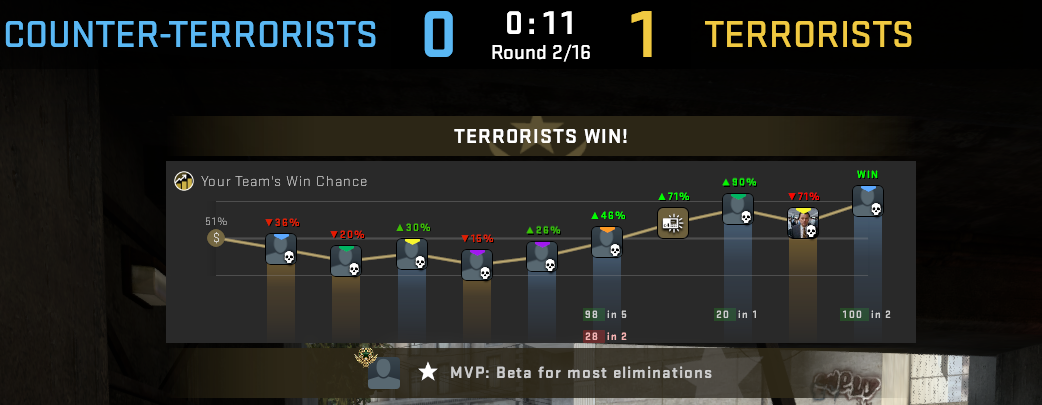
\includegraphics[width=.9\textwidth]{figures/jednanula}
 	\centering
 	\caption{Graf vyjadrujúci pravdepodobnosť víťazného tímu od firmy Valve \label{csgograf}}

 \end{figure}

 

\subsubsection{Využiteľné dáta hry Counter-Strike: Global Offensive :}

 \begin{itemize}
 	\item PlayerId - unikátne ID hráča
 	\item TeamId - unikátne ID tímu hráča
 	\item OpponentId - ID opozičného tímu
 	\item Round - počet hraných kôl
 	\item MapID - ID mapy
 	\item Kills - počet zabití
 	\item Assists - počet asistencií
 	\item Deaths - počet smrtí
 	\item Headshots - počet zabití streľbou do hlavy
 	\item EntryKills - počet prvých zabití v kole počas hry
 	\item Winner - víťaz
\end{itemize}
 

 

 \subsubsection{Vyhodnotenie Counter-Strike: Global Offensive}
 Pri vyhodnocovaní použiteľnosti hry sme sa pozerali na 3 oblasti. \\ \\ Potenciál/veľkosť publika a stávkovania. Efektívnosť využitia umelej inteligencie. Dostupnosť, respektíve využiteľnosť dát z hier. \\ \\
 Z hľadiska obecenstva, dostupnosti a možnosti stávkovania je CSGO veľmi lukratívna možnosť. Databáza hráčov je rozsiahla nielen v šírom počte, ale aj v rozmanitosti pôvodu hráčov, či už Európy, Ázie alebo Ameriky. Faktom je tiež, že ju spravuje firma Valve, ktorá má na starosti veľa iných hier a zároveň spracováva jednu z najväčších online platforiem pre virtuálnu knižnicu hier. \\
 Využiteľné dáta by sa skladali z predošlých stretnutí daných dvoch tímov, z aktuálnych informácií o jednotlivých hráčoch a ich štatistiky na vybraných mapách. Výhernosť tímu A proti tímu B a premostenie týchto informácií voči tímu C.\\
 Existuje ešte množstvo iných druhov dát, ktoré by zvýšili presnosť predikcie, ale sú to dáta, ktoré je možné zistiť už iba počas prebiehajúceho zápasu a vzhľadom na to, že stávky sa uzatvárajú pred začatím zápasu, sú tieto dáta nedostupné.
  Existuje ešte množstvo iných druhov dát, ktoré by zvýšili presnosť predikcie, ale sú to dáta, ktoré je možné zistiť už iba počas prebiehajúceho zápasu a vzhľadom na to, že väčšina stávok je pred začatím zápasu, tak sú tieto dáta nedostupné.
 \\ \\
 Potrebné dáta môžeme získať na stránke sportsdata. \footnote {
 https://sportsdata.io/developers/data-dictionary/csgo
}


\subsection{Dota 2}
Dota je jednou z dvoch najznámejších MOBA \footnote {
	MOBA - tip online hier s viacerými hráčmi, ktorí majú súboje v aréne
} hier na svete, s priemerným počtom hráčov viac ako 400 tisíc. \footnote{analýza hráčov Dota2 - https://steamcharts.com/app/570} Podobne ako Counter-Strike má predmety a verejný trh. Na druhej strane výherný rozpočet sa s ním nedá porovnať, pretože v roku 2021 prekonal 40 miliónov, čo je jeden z najväčších zo všetkých hier na svete. \footnote{prehľad všetkých turnajov a priceppolov - https://dota2.prizetrac.kr/}
\\ \\
Dota má nástroj na vyhľadávanie hier. Na obrázku \ref{dota1} si vieme vybrať šampiónov \footnote {
	šampión - postava, ktorú hráč reprezentuje v hre
} pre oba tímy a následne nám vybehnú zápasy, ktoré prebehli s týmito podmienkami.

 \begin{figure}[h!]
	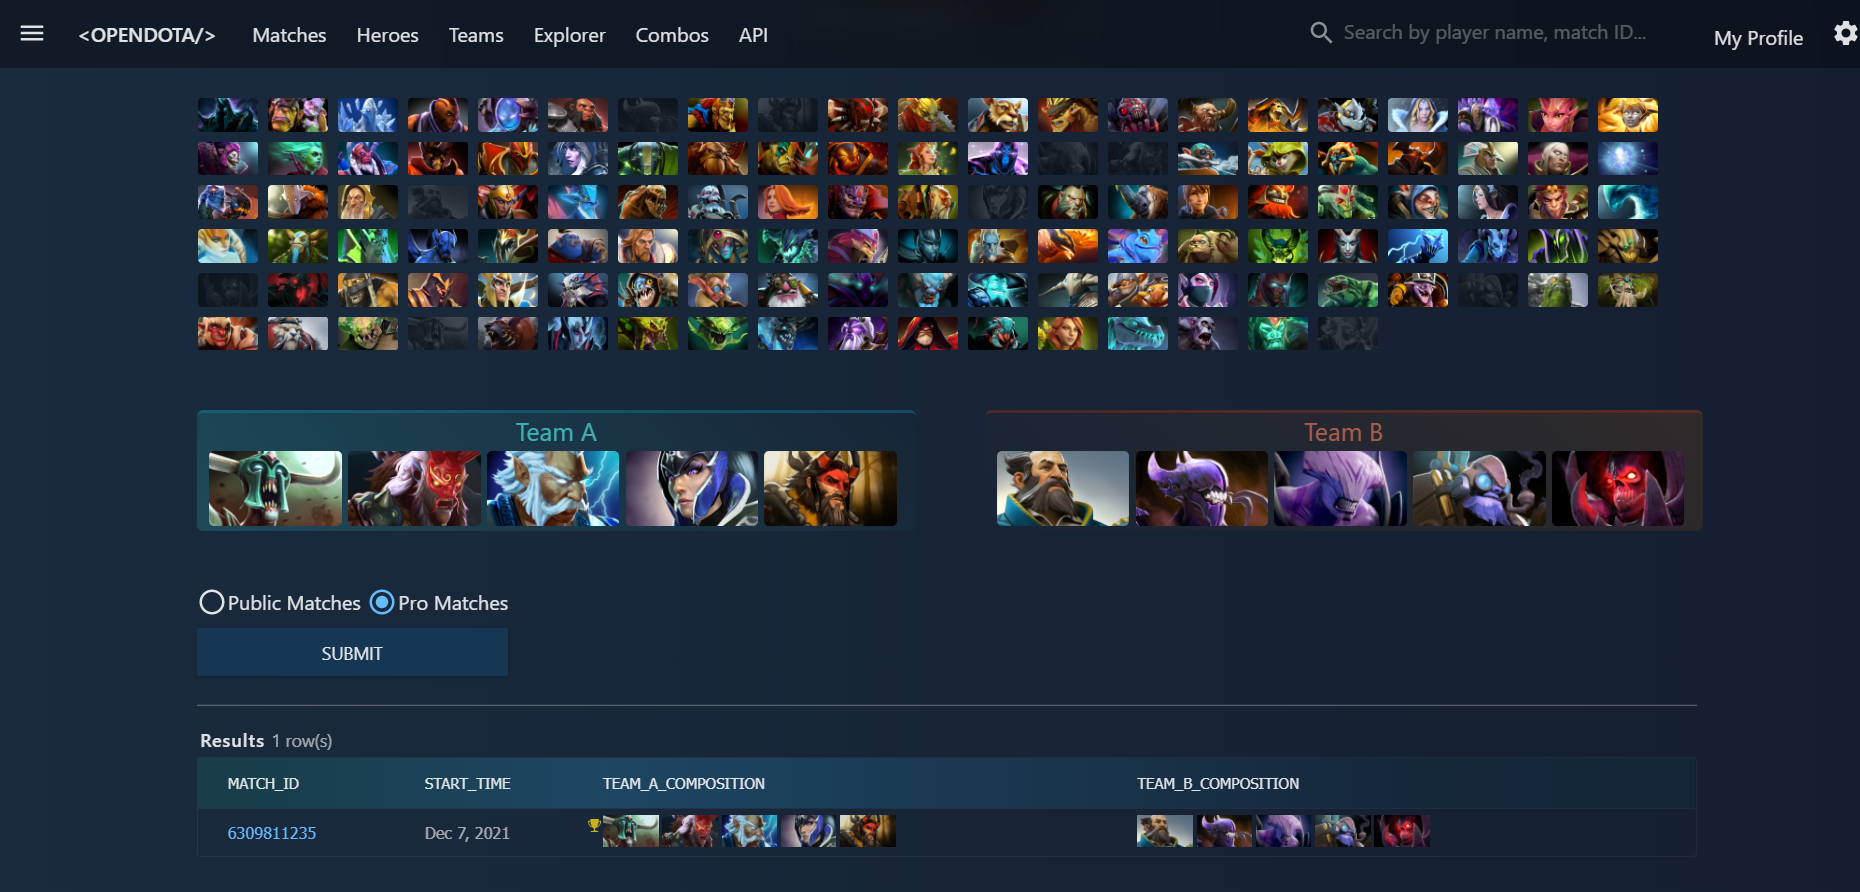
\includegraphics[width=.9\textwidth]{figures/dota1}
	\centering
	\caption{ dota1 \label{dota1}}
	
\end{figure}

Po rozkliknutí zápasu si v zázname vieme pozrieť výhercu a všetky informácie sprevádzajúce daný zápas, ako môžeme vidieť na obrázku \ref{dota2}.

 \begin{figure}[h!]
	
	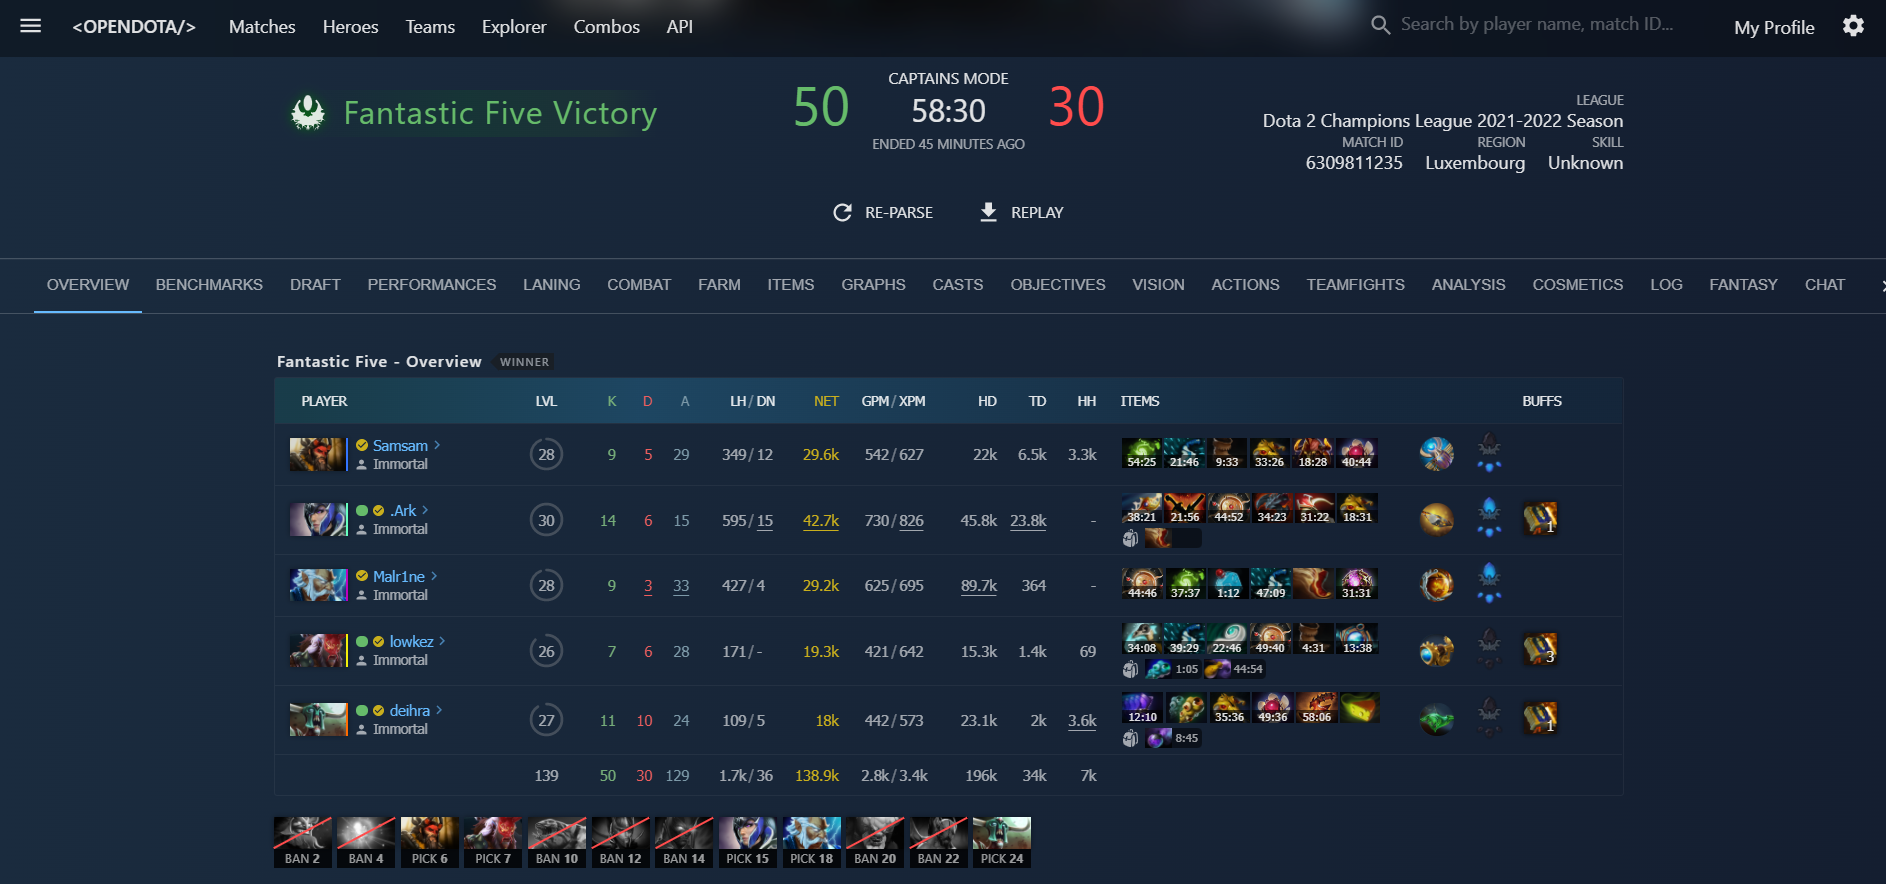
\includegraphics[width=.9\textwidth]{figures/dota2}
	\centering
	\caption{ dota2 \label{dota2}}
	
\end{figure}

\subsubsection{Využiteľné dáta hry Dota 2}

 \begin{itemize}
\item match\_id - unikátne ID zápasu 
\item duration - dĺžka zápasu 
\item radiant\_team\_id - ID radiant tímu 
\item radiant\_name - meno radiant tímu 
\item dire\_team\_id - ID dire tímu 
\item dire\_name - meno dire tímu 
\item leagueid - ID ligy
\item radiant\_score - skóre radiant
\item dire\_score - skóre dire
\item radiant\_win - výherca
\item radiant\_picks - radiant vybraní šampióni
\item radiant\_bans - radiant zabanovaní šampióni
\item dire\_picks - dire vybraní šampióni
\item dire\_bans - dire zabanovaní šampióni
\end{itemize}

\subsubsection{Vyhodnotenie hry Dota 2}
Znovu sa pozrieme na 3 oblasti. \\ \\ 
Publikum Doti a dosah je v porovnaní s CSGO nižší, na druhej strane jeho hráči sú odhodlaní brániť ju za každú cenu, čo môže mať negatívny, ale aj pozitívny efekt. Vzhľadom na  potenciál/veľkosť publika a stávkovania. Efektívnosť využitia umelej inteligencie a dostupnosť, respektíve využiteľnosť dát z hier.
\\ \\
Dáta pri Dote môžeme rozdeliť na dve kategórie : 
\\ \\
\begin{enumerate}
\item Dáta na predpoveď pred vybratím šampiónov - tieto dáta sú obmedzené z dôvodu, že nevieme, akých šampiónov budú dané dva tímy hrať. Takže sa spoliehame na predošlé výsledky daných dvoch tímov a ich stretnutí navzájom alebo s podobnými tímami. Takisto, ak sú noví hráči v tíme, vieme sa pozrieť aj na dáta individuálnych hráčov a na ich stretnutia z predošlých tímov. \\
Ďalšia podmienka, ktorou by sa dala predikcia vylepšiť, vychádza z porovnaní dát hráčov v danom tíme a šampiónov, ktorí sú práve v turnaji alebo sú v Patchi\footnote {
	Patch-aktuálna forma hry
} najviac hraní. Napríklad práve v rotácii najhranejších Carry šampiónov na profesionálnej scéne je daných 10 a týchto 10 porovnáme s hráčom v Carry pozícii, koľko má za nich nahraných profesionálnych hier alebo na ich SoloQ \footnote {
	SoloQ - zápasy odohrané na serveroch so všetkými hráčmi, aj neprofesionálnymi
} účte a ich výhernosť/penazí za minútu/KDA(zabitia, smrte, asistencie) s týmito šampiónmi.  
\\ \\
\item Dáta na predpoveď po vybratí šampiónov - týchto dát je kvantum, lebo vieme použiť dáta o šampiónoch nie len z profesionálnych hier, ale aj z hier normálnych hráčov z vyšších líg v pomere hodnotenia, inak povedaného hodnotiaceho rebríčka. Vedeli by sme použiť dáta aj z nižšie postavených hráčov Doty, ale to by s vysokou pravdepodobnosťou zhoršilo výsledok predikcie vzhľadom na fakt, že hra top 80 percent hráčov a hra top 0.003 percent hráčov sa nedá porovnať. Veľmi dôležité informácie by teda boli o výkonnosti šampiónov ako peniaze za minútu/zabitia/smrte/výhernosť. Zároveň by bolo veľmi zaujímavé skombinovať kompatibilnosť šampiónov spolu, spojením dvoch alebo viacerých šampiónov a ich spoločný priemerný winrate.
\end{enumerate}

\subsection{League of Legends}
League of Legends(Liga Legiend) je najrozšírenejšia MOBA hra na svete s viac ako 3 miliónmi každodenných používateľov a viac ako 100 miliónmi mesačných používateľov primárne z Číny, ako môžeme vidieť na grafe : \ref{leaguegraph} 

 \begin{figure}[h!]
	
	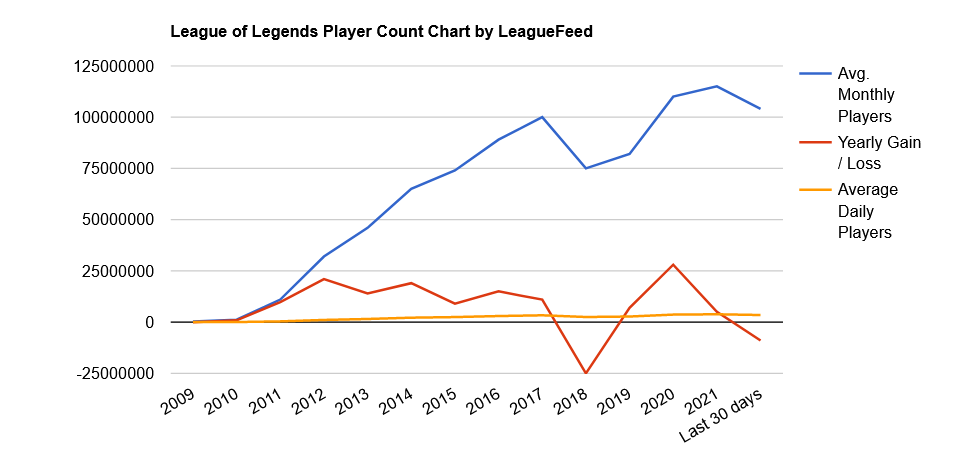
\includegraphics[width=.9\textwidth]{figures/leaguegraph}
	\centering
	\caption{ Graf znázorňujúci počet hráčov hry LOL  \label{leaguegraph}}
	
\end{figure}

Viac informácií nájdeme v článku \cite{leaguefeed}. 

Hra je z pohľadu tretej osoby a delí sa na dva tímy po piatich hráčoch. Víťazný tím je ten, ktorý zničí nepriateľskú základňu. Hráči zabíjaním nepriateľských minionov\footnote {
	minion - NPC (nastavený robot obmedzenej inteligencie vykonávajúci nejakú jednoduchú činnosť), ktoré sa snaží zničiť hocičo nepriateľské, čo je pred ním 
} dostávajú peniaze, ktoré môžu využiť na zlepšenie ich výzbroje, čo im dá väčšiu šancu na zabitie nepriateľa a následne nepriateľskej základne.
\\ 
Riot games má podobne ako Dota verejne dostupné informácie pre developerov na stránke developerov\footnote {
	https://developer.riotgames.com/
}.
a informácie o profesionálnych zápasoch na \footnote {https://lol.fandom.com/wiki/League\_Championship\_Series
}.

\subsubsection{Použiteľné dáta hry League of Legends}
\begin{itemize}
\item date - dátum zápasu 
\item blueteam - meno modrého tímu 
\item redteam - meno červeného tímu 
\item winner - víťaz 
\item bluebans - bany modrého tímu 
\item redbans - bany červeného tímu 
\item bluepicks - vybraní šampióni modrého tímu 
\item redpicks - vybraní šampióni červeného tímu 
\item blueroster - hráči modrého tímu 
\item redroster - hráči červeného tímu 
\end{itemize}
\subsubsection{Vyhodnotenie hry League of Legends}

Publikum z našich 3 hier ma LOL definitívne najväčšie, a to hlavne z dôvodu masívnej popularity v Číne, kde League of Legends má väčšiu popularitu a prestíž ako hocijaké iné, či už športy, hudba, tanec alebo spev. \cite{chinalol} 
\\
Aktuálne rozšírenie stávkovania na víťazný tím nie je vzhľadom na veľkosť publika až také rozšírené ako pri Dote a LOL. To môže ovplyvňovať aj fakt, že gambling je v Číne vysoko ilegálny, až na výnimky ako mesto Macau.\cite{chinagambling}
\\
Využitie  umelej inteligencie v hre LOL je veľké vzhľadom na verejne dostupné dáta a hlavne vysokú využiteľnosť.
\\
Dáta sú primárne veľmi podobné Dote, kde ich rozdeľujeme na dve časti, pred a po vybratí šampiónov.
\\
Veľmi lukratívne dáta, ktoré sú nanešťastie zatajené pred verejnosťou, sú dáta z hier, nazvané scrims. Pred oficiálnym začatím, napríklad svetového turnaja, sú všetky tímy zvolané a prítomné v usporiadajúcej krajine. Približne 3 týždne tieto tímy hrajú medzi sebou tréningové alebo kondičné zápasy, ktoré nie sú hodnotené, ale obsahujú veľa dôležitých informácií a taktík, ktoré tímy odskúšavajú. S prístupom k týmto dátam by sa dalo odskúšať veľa nových predikcií, ale k týmto dátam majú prístup len dané tímy a dáta sú vysoko chránené. Jedinou možnosťou, ako sa k nim dostať, by bol povolený prístup od tímov alebo odkúpenie za veľa peňazí.
\\


\section{Analýza dostupných spracovaní dát}
Časť analýzy dostupných spracovaní dát sa bude venovať jednotlivým druhom umelej inteligencie.

\subsection{Supervised learning}
Podkategória umelej inteligencie, ktorá používa dopredu označené dáta.  Používa tipy algoritmov\cite{umelainteligencia}
 \begin{itemize}
	\item Lineárna regresia - modeluje lineárny vzťah medzi atribútom a cieľovou premennou. Jej výstupom je tzv. spojitý výstup.\cite{regresia}
	\item SVM - algoritmus pomocných vektorových strojov alebo čiar. Je to rozšírenie perceptronu, jeho cieľ je maximalizovať hraničné pásmo \cite{svm}
	\item KNN - algoritmus k najbližších susedov je tzv. lenivý prístup, ktorý pri klasifikovaných dátach určuje triedu testovanej skupiny podľa toho, aký typ dát je najbližšie pri danej inštancii\cite{knn}
\end{itemize}

\subsection{Unsupervised learning}
Podkategória umelej inteligencie, ktorej dáta nie su dopredu klasifikované. 
\subsubsection{Používa metódy}
 \begin{itemize}
	\item Klastrovanie - pokúša sa nájsť skupiny podobných objektov, ktoré sú si podobné viac, ako objekty v iných skupinách\cite{clustering}
	\item Redukcia dimenzionality - je to proces, pri ktorom sa snažíme odstrániť počet nepotrebných premenných \cite{dimenzionalita}
\end{itemize}

\subsection{Reinforcement learning}
Časť umelej inteligencie, pri ktorej sa sledujú kroky inteligentných agentov na maximalizáciu efektívnosti dosiahnutia cieľa. Agenti sú zaradení do prostredia s limitovanými informáciami o danom prostredí, zároveň je im poskytnutá spätná väzba na kvalitu ich vykonaných krokov. \cite{reinforcement}
\subsubsection{Druhy agentov}
\begin{itemize}
	\item Reflexný agent - jeho nasledujúcu akciu zakladá na jeho aktuálnom poznaní sveta. Nehľadí na dôsledky jeho akcií.
	\item Cieľový agent - snaží sa dopredu naplánovať jeho potreby na dosiahnutie cieľa 
	\item Úžitkový agent 
\end{itemize}
\subsubsection{Vyhľadávacie algoritmy}
\begin{itemize}
	\item Brute force - používanie hrubej sily k dosiahnutiu požadovaného výsledku. To zahŕňa prechádzaním všetkých možností, až pokiaľ náhodou nedostaneme scenár, ktorý chceme.\cite{bruteforce}
	\item Backtracking - Algoritmus spätného vyhľadávania je algoritmom využívajúcim techniku CSP (Constraint satisfaction problem). Napríklad pri riešení problému N-Queens\footnote{N-Queens - problém, kde úlohou je rozložiť 8 dám na šachovnici bez toho, aby na seba navzájom útočili} tento algoritmus vyhľadá prázdne políčko v riadku šachovnice a hneď skontroluje, či daný stav porušuje pravidlá problému. Ak nájde políčko, kde stav neporušuje pravidlá problému, položí naň dámu a stav expanduje. Pri vyčerpaní dostupných políčok pre nasledujúce políčko sa algoritmus vráti na predchádzajúce políčko a daný stav zahodí.\cite{backtracking}
	\item Forwardcheck - Algoritmus doprednej kontroly je rozšírením algoritmu spätného vyhľadávania. Pri riešení problému N-Queens tento algoritmus využíva okrem spätného vyhľadávania aj doprednú kontrolu, kde po expandovaní stavu skontroluje, či sú aj ďalšie políčka v nasledujúcich riadkoch expandovateľné s pravidlami problému. Pri zlom riešení sa využije spätné vyhľadávanie. \cite{forwardcheck}
	\item Min-max konflikt - Algoritmus minimálnych konfliktov je algoritmom využívajúci techniku CSP (Constraint satisfaction problem). Pri riešení problému N-Queens tento algoritmus začína so stavom, kde všetky riadky obsahujú dámy, ale stále sa nejaké ohrozujú, vyberie si náhodnú dámu s konfliktami a skontroluje políčka v riadku, kde daná dáma sa nachádza. Ak nájde políčko s menším počtom konfliktov ako políčko, kde sa práve nachádza dáma, tak dámu na dané políčko presunie. Algoritmus končí úspešne po nájdení správneho stavu alebo neúspešne po určenom počte krokov.\cite{minmax}
\end{itemize}
